\section{Design Overview}
\label{s:design}

\Scrooge{} \textit{efficiently} implements the \CCC{} primitive, whilst remaining \textit{flexible} and \textit{robust} under failures. The design of \Scrooge{} is centered around three pillars:
\begin{enumerate}[wide,nosep,label=(P\arabic*),ref={P\arabic*}]

\item \label{g:zero} {\bf Efficiency.} In the common case, \Scrooge{} should send a single copy of the message to transmit cross-cluster, and no more than $n$ copies intra-cluster. This is the theoretical minimum to ensure that all nodes eventually receive the message.  There should be no additional communication. Moreover, any additional metadata sent as part of \Scrooge{} should have constant size.
\item \label{g:hetero} {\bf Generality.} \Scrooge{} must support \RSM{s} of arbitrary sizes, with diverse failure models and communication models, including crash/byzantine faults and both synchronous and asynchronous networks. Moreover, the protocol logic must work well for both traditional \BFT{} systems as well as newer Proof-of-Stake protocols, where a replica's share illustrates the weight its vote carries.

\item \label{g:failures} {\bf Robustness.} \Scrooge{} must remain robust to failures. Crashed or malicious replicas should have minimal impact on performance. There is a tension here: while the protocol should aggressively resend dropped messages
to minimize latency,  Byzantine nodes should not cause honest nodes to spuriously resend messages, as this can hurt throughput.
 
\end{enumerate}

\Scrooge{} leverages two observations: 1) the streaming nature of consensus, the protocol family at the core of any \RSM{} implementation, and 2) the fact that communication between replicated services is often long-running and full-duplex.
\Scrooge{} draws from the Transport Control Protocol's (TCP) approach to congestion control and message loss handling to guarantee \CCC{} with constant metadata overhead in the absence of failures.

\par \textbf{\CCC{} and congestion control}. TCP implements the abstraction of a reliable and ordered channel between two nodes. Two ideas are central to TCP's good performance: 1) leveraging full-duplex communication and 2) cumulative ACKing. In TCP, nodes simultaneously exchange messages. TCP leverages this bidirectional communication to piggy-back acknowledgements on the messages and minimize bandwidth requirements. Cumulative ACKing  then keeps these acknowledgements small: with a single counter $k$, a receiver informs a sender that it has received all packets with sequence number up to $k$. 
Receiving repeated counter values $k$ instead informs the sender that the packet with sequence number $k+1$ has likely been lost or delayed.

\Scrooge{}  draws inspiration from TCP and similarly leverages full-duplex communication and cumulative ACKing to lower overheads. However, unlike TCP, \Scrooge{} must 1) handle many-to-many communication as each RSM consists of multiple replicas 2) tolerate both crash and Byzantine failures. Dishonest replicas may lie about which message they have received, and can carefully time message drops to maximally hurt performance 3) efficiently handle nodes with different weights when dealing with stake-based BFT systems.
 

\begin{figure}[t]
    %\vspace{-6mm}
    \centering
    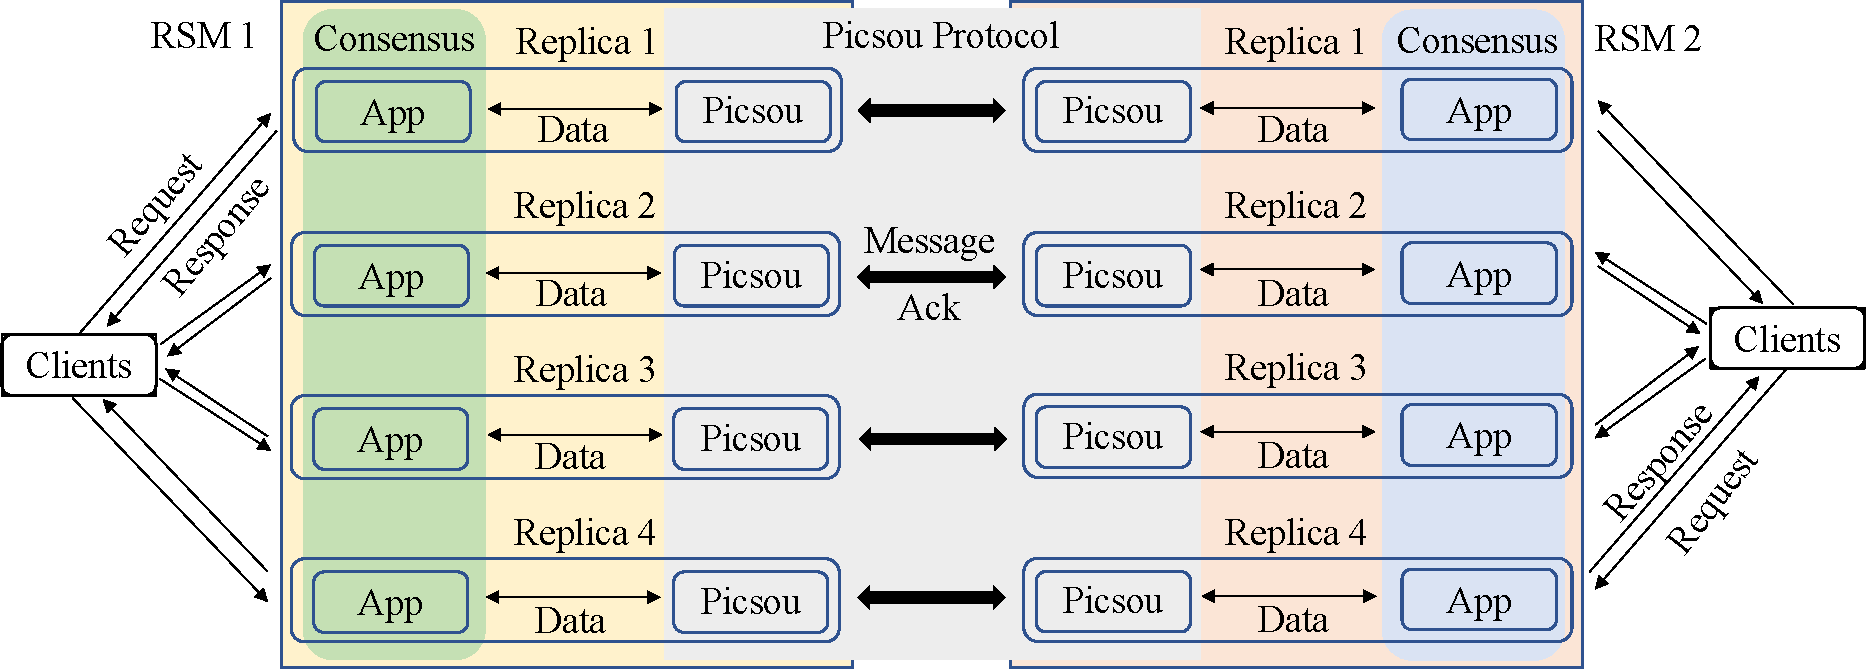
\includegraphics[width=0.85\columnwidth]{end-flow.pdf}
    %\vspace{-2mm}
    \caption{An illustration of \CCC{} primitive between two \RSM{s}, which employ some consensus protocol to manage their states and
    adopt \Scrooge{} for exchanging messages.}
    \label{fig:end-flow}
\end{figure}

\par \textbf{Overview.}  \Scrooge{}'s protocol logic can be  divided into the following logical steps, which we illustrate in Figure~\ref{fig:end-flow}.
\par (1) \textit{Consensus}:  On either side of \Scrooge{} lies a replicated state machine.  Each \RSM{} receives requests from clients and runs a consensus protocol (App) to commit these requests on each \RSM{} replica.
\par (2) \textit{Invoking \Scrooge{}}: Each replica forwards the committed request to the co-located \Scrooge{} library.
\par (3) \textit{Transmitting a message}: \Scrooge{} sends the message on behalf of the sending \RSM{}. In line with our stated efficiency goals, \Scrooge{} ensures that, in the absence of failures and during periods of synchrony, a \textit{single sender} forwards each request to a \textit{single replica} in the receiving \RSM{}. To minimize the risk of repeated failures caused by a faulty sender or receiver, \Scrooge{} carefully {\em rotates} sender-receiver pairs. In doing so, it ensures that every sender will eventually communicate with a correct receiver and vice-versa.
\par (4) \textit{Detecting successful or failed sends:} 
 \Scrooge{} must quickly determine whether a message has definitely been received (and can thus be garbage collected) or has definitely been dropped or delayed. 
Failure detection must be accurate to prevent failed nodes from causing spurious re-transmissions. The key challenge is disseminating this knowledge to all replicas when \Scrooge{} intentionally only sends messages pairwise for efficiency. To this effect, \Scrooge{} adapts TCP's cumulative acknowledgement approach to detect when messages have been received or dropped, even as malicious replicas can lie. These acknowledgements are piggy-backed on incoming messages, thus minimizing overhead. 
\par (5) \textit{Retransmissions}. When the protocol detects that a message has definitely been dropped, \Scrooge{} intelligently chooses the node responsible for resending the message. This is done without any communication across nodes. Unfortunately, without care, Byzantine nodes can selectively drop messages such that throughput craters. To address this issue, \Scrooge{}  includes (constant size) information about which messages have been lost, allowing the protocol to recover dropped messages in parallel. 
Traditional TCP can eschew this constraint as it assumes failures are rare and considers only point-to-point communication between nodes.


\begin{figure}[t]
    %\vspace{-6mm}
    \centering
    \begin{subfigure}[b]{0.32\columnwidth}
         \centering
         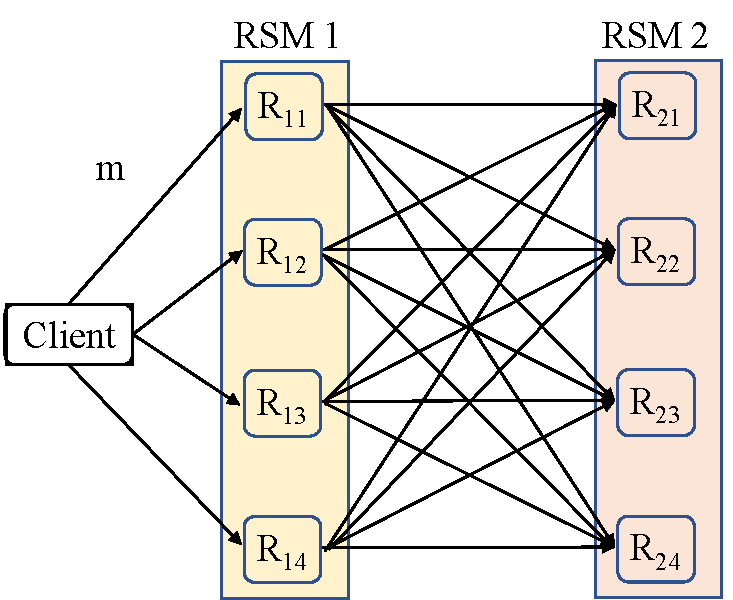
\includegraphics[width=\textwidth]{all-to-all.pdf}
         \caption{All-to-All}
         \label{fig:all-to-all}
     \end{subfigure}%
     \begin{subfigure}[b]{0.32\columnwidth}
         \centering
         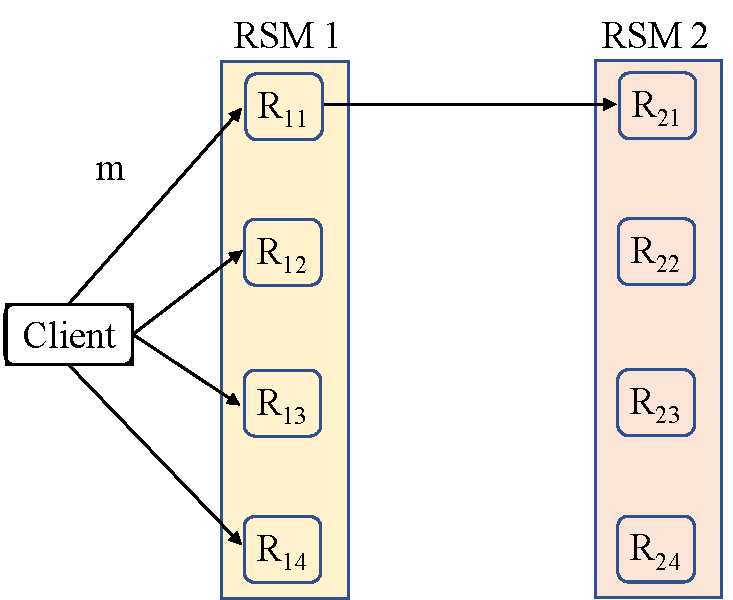
\includegraphics[width=\textwidth]{one-shot.pdf}
         \caption{One-Shot}
         \label{fig:one-to-one}
     \end{subfigure}%
     \begin{subfigure}[b]{0.32\columnwidth}
         \centering
         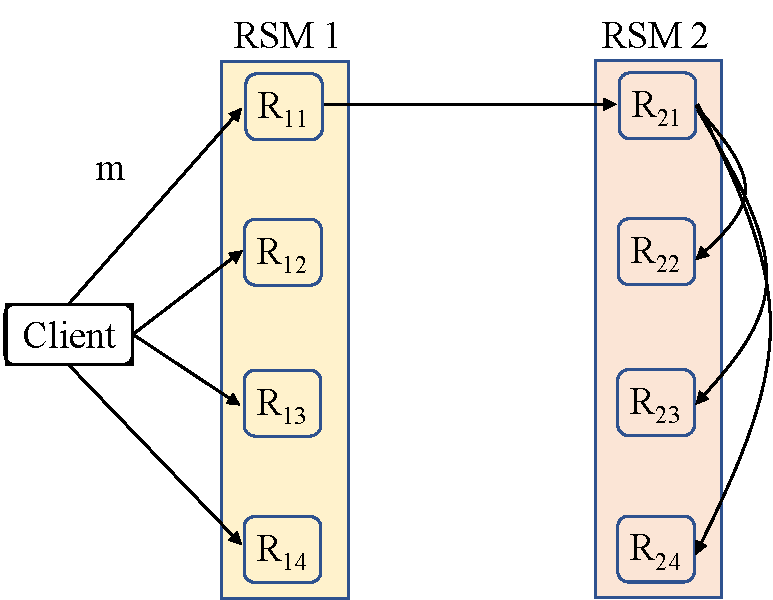
\includegraphics[width=1.05\textwidth]{scrooge.pdf}
         \caption{Picsou}
         \label{fig:scrooge}
     \end{subfigure}
    \caption{Comparison of the number of copies of a message $m$ sent across \RSM{s} by different \CCC{} protocols. 
    Note: One-Shot presents an incomplete design.}
    \label{fig:c3b-protocols}
\end{figure}


\par \textbf{Assumptions.} 
\Scrooge{} assumes knowledge of the current number of replicas in each RSM, failure thresholds, and stake distribution in the system (where applicable). \Scrooge{} further assumes that each request transmitted through \Scrooge{} is of the form $\SignMessage{m, \Seqn}{\Qusign{s}}$, 
where $m$ is a request committed at sequence number $\Seqn$ by a quorum of replicas in \RSM{} $\SMR{s}$. Each protocol sets a specific threshold $t$ above which the request has acquired sufficiently many signatures
$\Qusign{s}$ to be deemed committed. We further assume that all committed requests have contiguous sequence numbers.
\par \textbf{Correctness} We defer a full description of correctness and proofs to our submitted supplemental material.

\section{Protocol Design}

In this section, we describe the details of each logical step: transmitting a message, detecting successful/failed sends, and retransmissions. For simplicity, we ignore stake before revisiting our protocol when nodes have different shares (\S\ref{s:stake}). 
For clarity of exposition, while \Scrooge{} is bidirectional with RSMs acting as both the sender and the receiver, we describe the protocol as consisting of a sender RSM and a receiver RSM. In reality, the protocol is mirrored.

We start by describing \Scrooge{}'s behaviour in the common-case (\S\ref{ss:failurefree}) before considering failures (\S\ref{ss:failures}). 



\begin{figure}[t]
    %\vspace{-6mm}
    \centering
    \begin{subfigure}[t]{0.494\columnwidth}
         \centering
         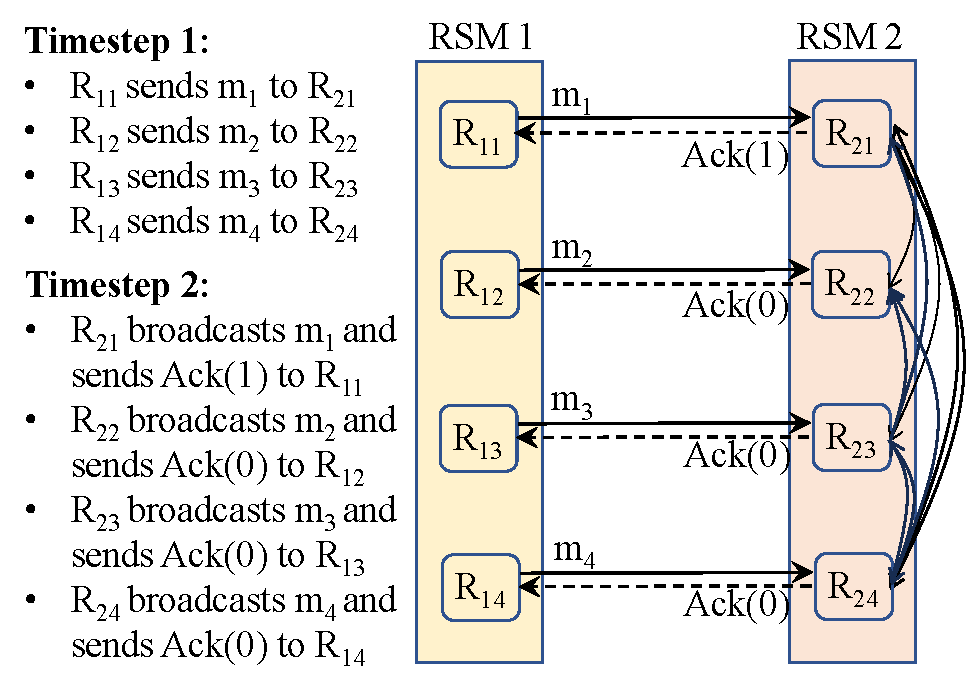
\includegraphics[width=\columnwidth]{acking-p1.pdf}
         %\caption{First set.}
         \label{sfig:first}
     \end{subfigure}
     \begin{subfigure}[t]{0.494\columnwidth}
         \centering
         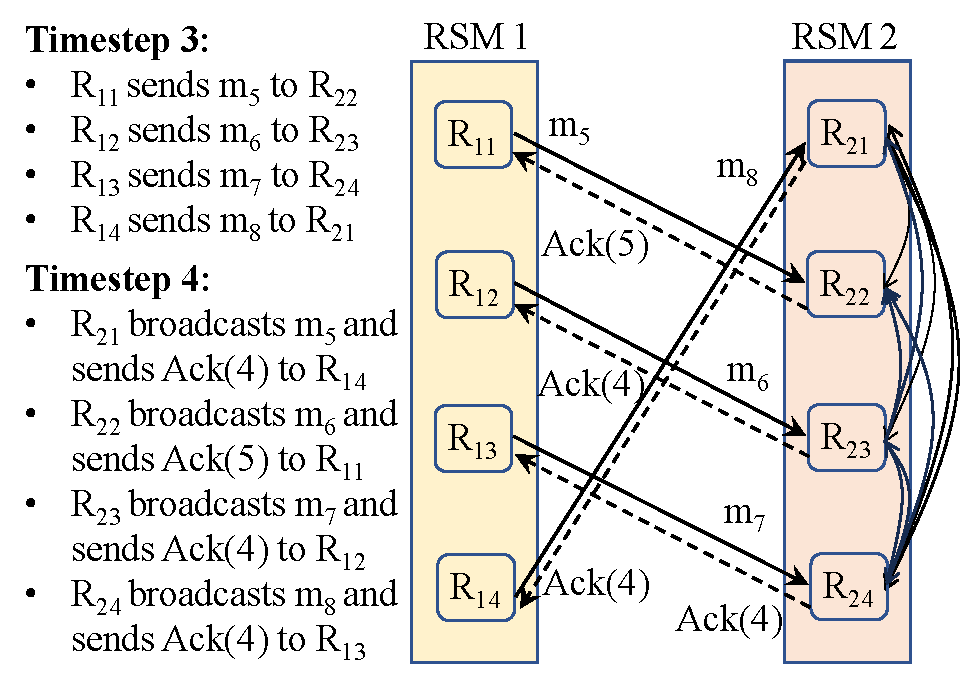
\includegraphics[width=\columnwidth]{acking-p2.pdf}
         %\caption{Second set.}
         \label{sfig:second}
     \end{subfigure}%
    \caption
    {Example failure-free run in \Scrooge{}}
    %This figure illustrates how sender \RSM{} (\RSM{} $1$) forwards messages to receiver \RSM{} (\RSM{} $2$) using \Scrooge{} protocol.
    %Assume the sequence number for messages starts from $1$. 
    %Each \RSM{} $1$ replica sends (round robin) its designated message to a specific replica of \RSM{} $2$. 
    %In turn, it receive a cumulative acknowledgment.
    \label{fig:round-robin}
\end{figure}


\subsection{Failure-free behaviour}
\label{ss:failurefree}

\par \textbf{Sending a message.} \Scrooge{}'s send logic has three goals: 1) minimize the number of nodes sending the same message, 
2) maximize the chances that a message will be successfully transmitted quickly, 
and 3) asynchronously disseminate any knowledge of received messages to all other nodes. 
\Scrooge{} achieves these goals
by partitioning, round-robin, the set of requests to send across all replicas in the sending \RSM, 
and rotating receiver nodes  every round.

By the definition of an \RSM{}, each replica contains a log of committed requests. 
\Scrooge{} evenly partitions the task of transmitting a committed message across all replicas such that each message is sent by a single node: the $l$-th \Scrooge{} node sends messages with sequence number $(\Seqn \bmod \n{s} \equiv l)$. 
Each replica rotates its choice of receiver on every send: if $\n{r}$ is the total number of receivers in the receiver \RSM{}, 
and $j$ is the identifier of the previous recipient, then the $l$-th sender will send to receiver replica $(j+1) \bmod \n{r}$. 
%\rfr{We could also just say node $j$ would send $\Seqn$ to $j+\lfloor\frac{\Seqn}{\n{s}}\rfloor \bmod \n{r}$}.

Rotating sender-receiver pairs in this way guarantees that every pair of replicas will eventually exchange messages and ensures that (1) information about the state of each node is propagated to every other node in the system, and (2) no sender is continuously sending to a faulty replica (or vice-versa). This process is also essential to bounding the number of re-transmissions needed in the presence of failures (more detail in \S\ref{ss:failures}). As is standard in TCP, we allow senders to transmit a window of messages in parallel.
%
%\begin{figure}[h]
%    \begin{myprotocol}
%        \INITIAL{Initialization:}{\newline
%	{%\color{orange}
%	// Let $\MAck{}$ be the list of received messages sorted by sequence number.
%	}}
%	\vspace{1mm}
%
%        \TITLE{Sender-role}{at the $j$-th \Scrooge{} instance at replica $j$}
%        \IF{Message $m$ with sequence $\Seqn$ is such that $k \bmod j = 0$}
%            \IF{$i$ is the identifier of previous receiver replica of receiver \RSM{} $\SMR{r}$}
%                \STATE $rid$ $:=$ $(i+1) \bmod \n{r}$
%                \STATE Send $\SignMessage{m, \Seqn}{\Qusign{s}}$ to receiver with identifier $rid$.
%                \STATE $\{m', p \} :=$ Message with highest sequence $p$ such that $\MAck{}$ has a message for each sequence number $\le p$.
%                \STATE Piggyback $\Ack{p}$ with message $\SignMessage{m, \Seqn}{\Qusign{s}}$.
%            \ENDIF
%        \ENDIF
%        \SPACE
%
%        \TITLE{Receiver-role}{at the $i$-th \Scrooge{} instance at replica $i$}
%        \EVENT{Received message $\SignMessage{m, \Seqn}{\Qusign{s}}$ from $j$-th replica of \RSM{} $\SMR{s}$}
%            \STATE Broadcast $\SignMessage{m, \Seqn}{\Qusign{s}}$ in its \RSM{} $\SMR{r}$.
%            \STATE Add $\{m, \Seqn \}$ to list $\MAck{}$.
%        \ENDEVENT
%    \end{myprotocol}
%    \caption{\Scrooge{} code running at the sender and receiver replicas.\nc{We need to be consistent with pseudocode and text}}
%    \label{alg:scrooge-no-fail}
%\end{figure}
%%


\par \textbf{} Upon receiving a message, the $j$-th replica $\Replica{r}{j}$ checks that the message $\SignMessage{m, \Seqn}{\Qusign{s}}$ is valid (the message has provably been committed by the sender \RSM{}) and if so, broadcasts it to the other nodes in its \RSM{}.  In the failure-free case,
\Scrooge{} thus sends a total of $\n{r}$ messages. This is in line with the theoretical minimum of all \CCC{} protocols.

\begin{figure}[t]
    %\vspace{-6mm}
    \centering
    \begin{subfigure}[b]{0.32\columnwidth}
         \centering
         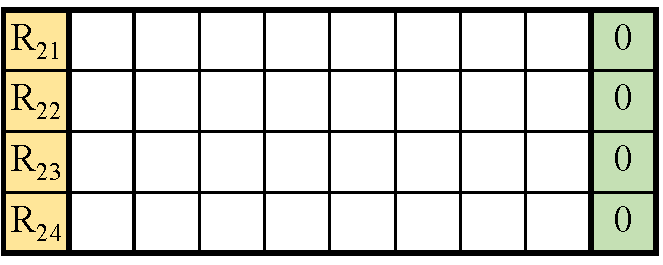
\includegraphics[width=\textwidth]{cack1.pdf}
         \caption{Initial}
         \label{sfig:initial}
     \end{subfigure}
     \begin{subfigure}[b]{0.32\columnwidth}
         \centering
         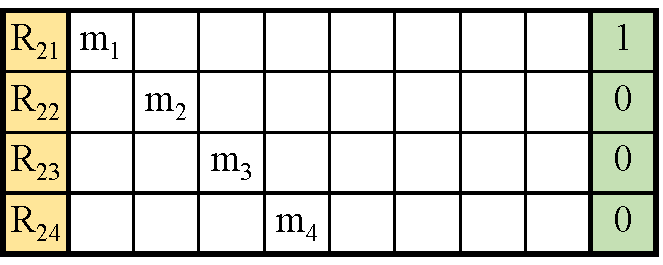
\includegraphics[width=\textwidth]{cack2.pdf}
         \caption{Timestep 1}
         \label{sfig:first-set}
     \end{subfigure}
     \begin{subfigure}[b]{0.32\columnwidth}
         \centering
         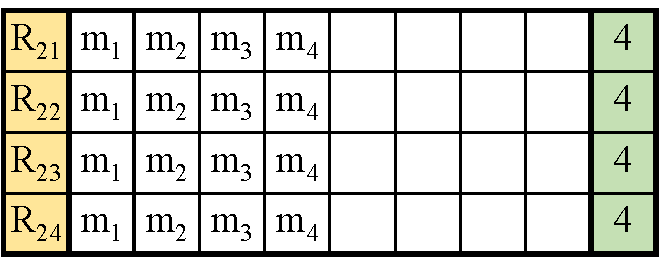
\includegraphics[width=\textwidth]{cack3.pdf}
         \caption{Timestep 2}
         \label{sfig:first-broadcast}
     \end{subfigure}
     \begin{subfigure}[b]{0.32\columnwidth}
         \centering
         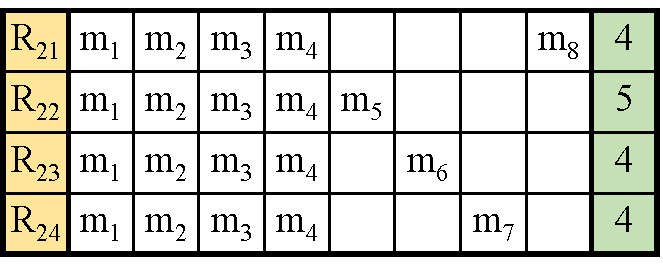
\includegraphics[width=\textwidth]{cack4.pdf}
         \caption{Timestep 3}
         \label{sfig:second-set}
     \end{subfigure}
     \begin{subfigure}[b]{0.32\columnwidth}
         \centering
         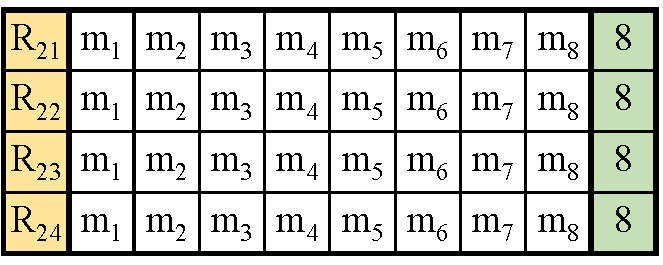
\includegraphics[width=\textwidth]{cack5.pdf}
         \caption{Timestep 4}
         \label{sfig:second-broadcast}
     \end{subfigure}
    \caption{Receiver's view of events in Figure~\ref{fig:round-robin}.}
    \label{fig:ack-counter}
\end{figure}

We illustrate \Scrooge's logic in Figure~\ref{fig:round-robin}.
Note that, in each time-step, we assume that a replica completes all the relevant tasks in parallel. Consider a system
with $\n{r} = 4$ replicas ($\uf{}= \rf{} = 1$).
In Timestep 1, replicas $\Replica{1}{1}$, $\Replica{1}{2}$, and $\Replica{1}{3}$
of $\RSM{}_1$ send messages
 $m_1$, $m_2$, and $m_3$ respectively to receivers $\Replica{2}{1}$, $\Replica{2}{2}$, and $\Replica{2}{3}$. 
In Timestep 2 \nc{1?}, these replicas internally broadcast these messages to the other nodes
in their \RSM{}.
Concurrently, $\Replica{2}{1}$, $\Replica{2}{2}$, and $\Replica{2}{3}$ acknowledge receipt of these messages and send $\Ack{1}$, $\Ack{0}$, and $\Ack{0}$ to senders 
$\Replica{1}{1}$, $\Replica{1}{2}$, and $\Replica{1}{3}$.
We discuss acknowledgements later in the section.
In Timestep 3, $\Replica{1}{1}$, $\Replica{1}{2}$, and $\Replica{1}{3}$ rotate receivers and
send messages $m_5$, $m_6$, and $m_7$ to $\Replica{2}{2}$, $\Replica{2}{3}$, and $\Replica{2}{4}$.
In Timestep 4, these replicas once again broadcast the received messages to the other nodes in their \RSM{}.
Simultaneously, $\Replica{2}{1}$, $\Replica{2}{2}$, and $\Replica{2}{3}$ send $\Ack{4}$, $\Ack{5}$, and $\Ack{4}$ to senders 
$\Replica{1}{4}$, $\Replica{1}{1}$, and $\Replica{1}{2}$, respectively. 
\par \textbf{Detecting successful sends.} To guarantee correctness, all committed messages must eventually be received by an honest node in the receiving \RSM{}. The sending \RSM{} must thus detect when its message has \textit{definitely} been received by an honest node. Specifically, all honest nodes in the sending \RSM{} (not just the sender) must learn that a message was successfully delivered. This is necessary to preclude honest nodes from unnecessarily resending messages.

There are three primary challenges: (1) malicious nodes may lie about the set of messages received, (2) for efficiency, \Scrooge{} should not require nodes within an \RSM{} to exchange information beyond the necessary message broadcast, and (3) any additional metadata should be small. \Scrooge{} realizes these goals through \textit{cumulative quorum acknowledgements} (or \quack{}s). A cumulative quorum acknowledgement with value $\Seqn$ proves to the sending \RSM{} that all messages with sequence number up to $\Seqn$ have been received by at least one honest replica. 

More specifically, each replica, upon receiving a message with sequence number $\Seqn$, inserts it into a sorted list containing all previously received messages. The replica does not, however, \textit{selectively} acknowledge $m_k$. Instead, it identifies the highest message $m_p$ in the list for which all messages with a smaller sequence number have been received. The replica crafts an acknowledgement $\Ack{p}$ that cumulatively acknowledges receipt of messages $0$ to $p$. \Scrooge{} takes advantage of the full-duplex nature of the protocol to piggy-back these acknowledgements onto the messages that the receiving \RSM{} is itself sending to the sending \RSM{}. If no such message exists, the \RSM{} sends a no-op.
%Note \msg{Not sure if this sentence will be clear to a reader. At present it seems like some senders may not receive cumulative acknowledgment?}\mnc{Fair point. Happy to remove}
%that this implies that the acknowledgement for message $p$ may not be sent back to the initial sender of $p$, but to another replica in the sending \RSM{}.

On the sender side, each replica eventually receives messages and acknowledgements from all $\n{r}$ receiving replicas, thanks to \Scrooge{}'s round-robin strategy.  Each replica maintains an $\n{r}$ sized array that summarizes the highest acknowledgement received from each replica of the receiving \RSM{}. There exists a \quack{} for message $m_p$ (we say message $m_p$ has been \quack{}ed) if at least $\uf{r} + 1$ array entries have a value greater or equal to $p$, which indicates that $\uf{r}+1$ replicas have acknowledged receipts of all messages up to $p$. As there are only $\uf{r}$ failed replicas, one of these replicas must be honest. We thus have the guarantee that this correct replica will broadcast the message to all other remaining honest participants. Note that \Scrooge{} additionally uses MACs when configured to handle Byzantine failures ($\rf{}>0$)
%\begin{figure}[h]
%    \begin{myprotocol}
%        \INITIAL{Initialization:}{\newline
%	{%\color{orange}
%	// Let $\QuArr{}$ be the array of $\n{r}$ size.\newline
%        // Let $\highest$ be the largest \quack{ed} value 
%	}}
%	\vspace{1mm}
%
%        \EVENT{Received $\Ack{p}$ from $i$-th replica of \RSM{} $\SMR{r}$}
%            \STATE Set $\QuArr{i} := p$.
%            \WHILE{true}
%                \IF{$\f{r} + 1$ entries of $\QuArr{}$ have value $\ge \highest + 1$}
%                    \STATE Garbage collect message with sequence number $\highest$
%                    \STATE $\highest ++$
%                \ELSE
%                    \STATE break;
%                \ENDIF
%            \ENDWHILE
%        \ENDEVENT
%    \end{myprotocol}
%    \caption{Cumulative quorum acknowledgments at sender.}
%    \label{alg:scrooge-no-fail}
%\end{figure}
%

\par \textbf{Example.} To illustrate our message \quack{}ing logic, 
we continue with our example in Figure~\ref{fig:round-robin}.
Figures~\ref{fig:ack-counter} and ~\ref{fig:quack-counter} describe the protocol logic for, respectively, the receiver RSM and the sender RSM.  
Each row in Figure~\ref{fig:ack-counter} summarizes the sorted list of messages received at each replica, 
with the last column denoting the highest cumulative acknowledgment for this node.
Initially, all lists are empty and cumulative acknowledgment values are all set to $0$ (\ref{sfig:initial}). 
At Timestep 1, 
receivers $\Replica{2}{1}$, $\Replica{2}{2}$, and $\Replica{2}{3}$ (\ref{sfig:first-set}) store messages $m_1$, $m_2$ and $m_3$.
$R_{21}$'s cumulative acknowledge counter thus increases to 1, while others stay at 0 as they are still missing $m_1$. 
$\Replica{2}{1}$, $\Replica{2}{2}$, and $\Replica{2}{3}$ thus send $\Ack{1}$, $\Ack{0}$ and $\Ack{0}$ to the sender RSM.
At Timestep 2, each receiver, thanks to the internal broadcast mechanism, receives all three messages. All cumulative acknowledgement counters thus go to $4$ (\ref{sfig:first-broadcast}). By Timestep 3, receivers $\Replica{2}{1}$, $\Replica{2}{2}$, and $\Replica{2}{3}$ have all received $m_8$, $m_5$ and $m_6$.
$\Replica{2}{2}$ has received messages $m_1$ to $m_5$, and thus updates its cumulative acknowledgement to $5$. In contrast,
through $\Replica{2}{1}$ and $\Replica{2}{3}$ have received messages $m_8$ and $m_6$ respectively, they are missing $m_5$ and thus cannot
yet update their cumulative acknowledgement counter. Each replica sends $\Ack{4}$, $\Ack{5}$ and $\Ack{4}$ back to the sending RSM.
Finally, at Timestamp 4, the internal broadcast mechanism disseminates all these messages; each replica can update its cumulative acknowledgement to 8, and send $\Ack{8}$ back to the initiating RSM. 

Consider instead the protocol logic at the sender-side (Figure~\ref{fig:quack-counter}), which processes these cumulative acknowledgements and determine when a \quack{}
has formed. Each replica maintains an array summarising how many acknowledgements have been received for each message. A message is \quack{}ed at a replica if this replica receives $\uf{}+1=2$ acknowledgements for $m$.
 Initially, \quack{} counters at each replicas are empty (\ref{sfig:init-ack}). At Timestamp $2$, $\Replica{1}{1}$
(\ref{sfig:first-ack})'s records that it has received an acknowledgement for $m_1$  ($\Ack{1}$) from $\Replica{2}{1}$. 
At Timestamp 4, (\ref{sfig:second-ack}), $\Replica{1}{1}$ receives $\Ack{5}$ from $\Replica{2}{2}$. It updates its local array
to reflect that it now has received two acknowledgements for $m_1$, and \quack{}s $m_1$. It further reflects receipt of acknowledgements
for $m_2$, $m_3$, $m_4$, and $m_5$. $\Replica{1}{2}$ and $\Replica{1}{3}$ similarly indicate that they have received acks for $m_1$, $m_2$, $m_3$, and $m_4$
as they both received $\Ack{4}$. 

\begin{figure}[t]
    %\vspace{-6mm}
    \centering
    \begin{subfigure}[b]{0.32\columnwidth}
         \centering
         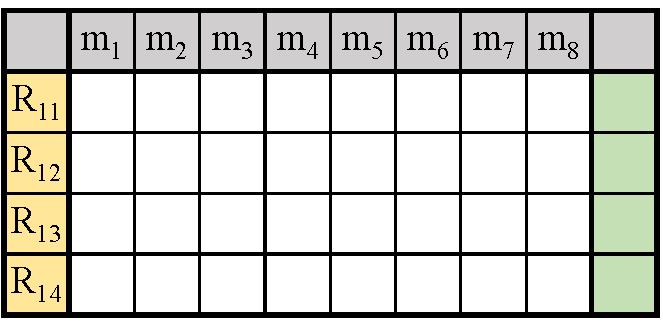
\includegraphics[width=\textwidth]{quack1.pdf}
         \caption{Initial}
         \label{sfig:init-ack}
     \end{subfigure}
     \begin{subfigure}[b]{0.32\columnwidth}
         \centering
         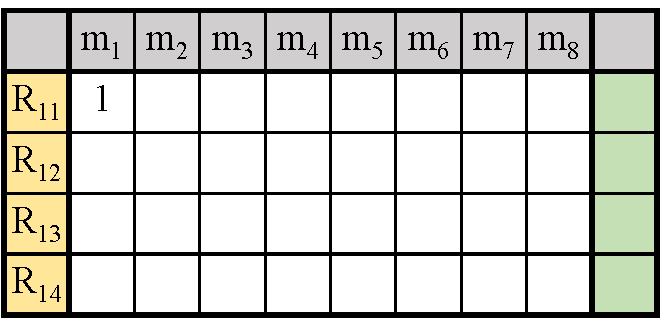
\includegraphics[width=\textwidth]{quack2.pdf}
         \caption{Timestep 2}
         \label{sfig:first-ack}
     \end{subfigure}
     \begin{subfigure}[b]{0.32\columnwidth}
         \centering
         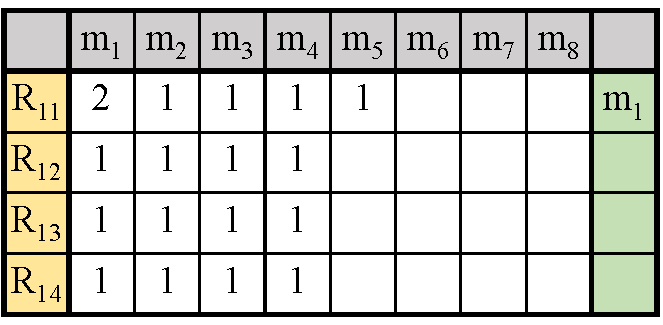
\includegraphics[width=\textwidth]{quack3.pdf}
         \caption{Timestep 4}
         \label{sfig:second-ack}
     \end{subfigure}
    \caption{Sender's view of events in Figure~\ref{fig:round-robin}.}
    \label{fig:quack-counter}
\end{figure}

\par \textbf{Summary} The joint techniques of full-duplex communication, cumulative acking, and rotation of sender/receiver pairs allows \Scrooge{} to ensure that all replicas in an \RSM{} will eventually learn that all committed requests have been reliably received by the receiving \RSM{}. In line with its efficiency goals, the protocol achieves this with only two additional counters, and with no additional communication between the replicas of an \RSM{} beyond the necessary broadcast.  The use of \quack{}s is key to \Scrooge{}'s generality: they require no synchrony assumptions and simply require that the sending \RSM{} know the failure threshold of the receiving \RSM{}. 

\subsection{Handling Failures}
\label{ss:failures}
Crashed replicas can fail to complete a send or broadcast; byzantine replicas can either intentionally drop messages (whether when sending or receiving) or lie in their acknowledgements. They can, for instance, spuriously advance their ack, thus potentially causing honest senders to believe that their message has been received, or, on the contrary, send an intentionally low ack, causing honest replicas to spuriously resend messages.  \Scrooge{} must effectively handle these failures without sacrificing correctness or performance. To this effect,  \Scrooge{} must quickly and reliably detect \textit{when} a message has \textit{definitely} been dropped and quickly retransmit it. The system must do so without any additional intra or inter-\RSM{} communication beyond resending the message itself. 

\par \textbf{Detecting definitely failed sends.} The protocol once again leverages \quack{}s.   Recall that all sender replicas eventually obtain a \quack{} for every message that has \textit{definitely} been delivered. One can instead leverage duplicate 
\quack{}s to determine when an honest replica has \textit{definitely not} received a specific message. 
In more detail, let us assume that a \quack{} for message $m_k$ has formed at $\Replica{s}{l}$. 
This \quack{} indicates that at least $\uf{} + 1$ (at least one honest) replicas have received every message up to message $m$ with sequence number $k$.  
If one of these replicas sends a duplicate acknowledgement $\Ack{k}$ for $m$, one can conclude that this replica claims to not have received message at sequence number $k + 1$. Once a duplicate \quack{} forms for the $k$-th message at replica $\Replica{s}{l}$,  $\Replica{s}{l}$ can reliably infer that $(k+1)$-th message has been lost or delayed as an honest replica is complaining about the missing message. All other honest replicas of the sending \RSM{} $\SMR{s}$ will eventually receive a duplicate \quack{} and thus detect the failed exchange.
The use of the Upright failure model, which distinguishes malicious failures $\rf{}$ from all other failures, allows us to reduce the size of the duplicate \quack{}: while the initial \quack{} is of size    $\uf{} + 1$, duplicate \quack{}s must be of size $\rf{} + 1$ as they must be large enough to preclude actively malicious nodes from triggering spurious resends. In contrast, a faulty node (one that will eventually crash) sending a duplicate acknowledge still signals the existence of a faulty sender/receiver or dropped message. As such, in a system with only crash failures (when $\rf{}=0$), a single duplicate \Ack{} is sufficient to trigger a message resend.

\par \textbf{Retransmitting the dropped message.} Upon detecting a failed send, the message must be quickly retransmitted. Just as a single replica was responsible for sending the initial message, \Scrooge{} ensures that a single replica is "elected" as the retransmistter. It does so \textit{without} requiring additional communication between replicas. The protocol logic hinges on three observations: 1) all correct replicas know about all the messages that must be transmitted (by definition of an \RSM{}) and know who initially sent the message, 2) all correct replicas eventually learn about which messages have been \quack{}ed,
3) the number of repeated \quack{}s indicate the number of failed retransmissions. 
\Scrooge{} uses this information to compute the ID of the retransmitter as: $sender_{new} = sender_{original} + (\#_{retransmit} \mod \n{sender})$.  Each honest replica computes this function, and retransmits the message if its ID matches $sender_{new}$.  Each retransmission round thus has a single sender.


\begin{figure}[t]
    %\vspace{-6mm}
    \centering
    \begin{subfigure}[b]{0.3\columnwidth}
         \centering
         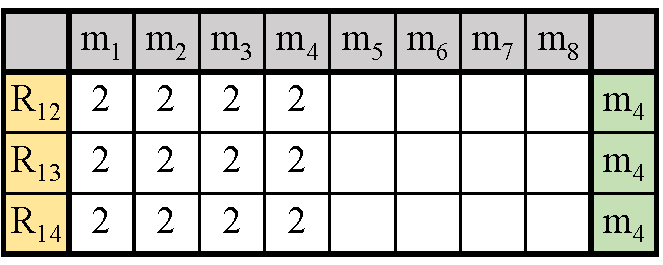
\includegraphics[width=\textwidth]{fail-quack1.pdf}
         \caption{Timestep 6}
         \label{ssfig:init-ack}
     \end{subfigure}
     \begin{subfigure}[b]{0.3\columnwidth}
         \centering
         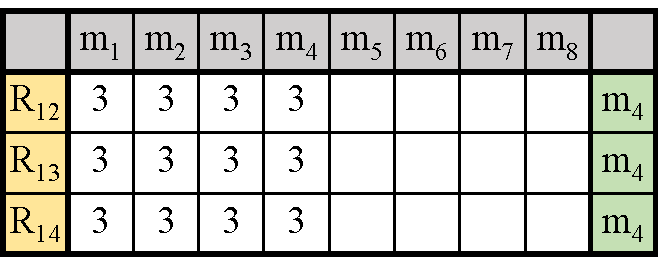
\includegraphics[width=\textwidth]{fail-quack2.pdf}
         \caption{Timestep 8}
         \label{ssfig:first-ack}
     \end{subfigure}
     \begin{subfigure}[b]{0.3\columnwidth}
         \centering
         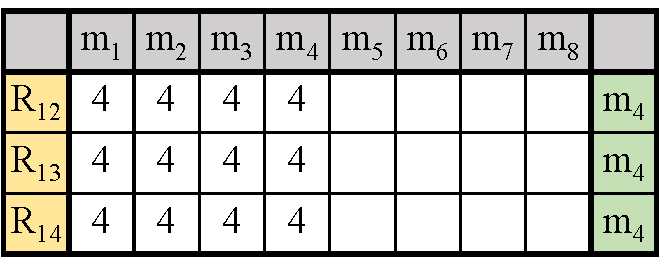
\includegraphics[width=\textwidth]{fail-quack3.pdf}
         \caption{Timestep 10}
         \label{ssfig:second-ack}
     \end{subfigure}

     \begin{subfigure}[b]{0.3\columnwidth}
         \centering
         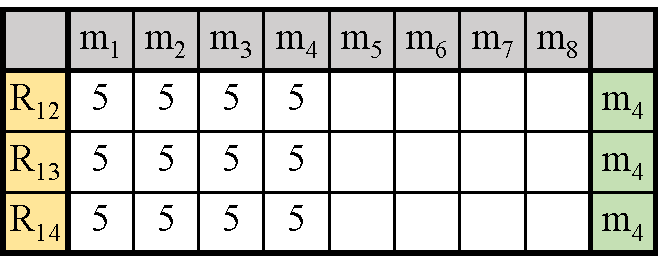
\includegraphics[width=\textwidth]{fail-quack4.pdf}
         \caption{Timestep 12}
         \label{usfig:init-ack}
     \end{subfigure}
     \begin{subfigure}[b]{0.3\columnwidth}
         \centering
         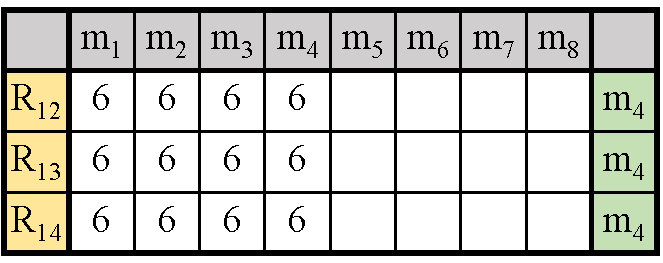
\includegraphics[width=\textwidth]{fail-quack5.pdf}
         \caption{Timestep 14}
         \label{usfig:first-ack}
     \end{subfigure}
     \begin{subfigure}[b]{0.3\columnwidth}
         \centering
         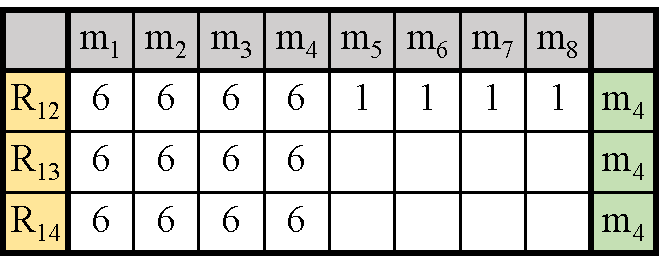
\includegraphics[width=\textwidth]{fail-quack6.pdf}
         \caption{Timestep 16}
         \label{usfig:second-ack}
     \end{subfigure}
    \caption{Sender's view of events if replica $\Replica{1}{1}$ fails after Timestep 2 (does not send any message after $m_1$) in Figure~\ref{fig:round-robin}. }
    \label{fig:fail-quack-counter}
\end{figure}

To illustrate, consider once again our initial example (Figure~\ref{fig:round-robin}), but this time, let us assume that sender replica $\Replica{1}{1}$ fails after sending message $m_1$ but before sending messages $m_5$ and $m_9$. As a result, no receiver receives these messages. In Figure~\ref{fig:fail-quack-counter}, we timestep through this failure scenario. For simplicity of exposition, we assume that senders (except $\Replica{1}{1}$) send new messages in odd timesteps and receive cumulative acknowledgements in even timesteps. 
%
As $\Replica{1}{1}$ fails after sending $m_1$ (at the end of Timestep 4) every other replica of \RSM{1} receives cumulative acknowledgment 
message $\Ack{4}$ for the first time (Figure~\ref{fig:round-robin}).
These senders continue sending remaining messages, so by Timestep 6, all senders
have received  $\Ack{4}$ messages twice (from $\uf{r}+1 =2$ receivers). This allows them to mark messages $m_1$ to $m_4$ as \quack{ed}. 
These receivers cannot acknowledge any message greater than $m_4$ as they are yet to receive $m_5$.
The senders are yet to receive $\Ack{4}$ messages from the remaining replicas (in our case $2$ other replicas).
They receive these acknowledgments during Timesteps 8 and 10. 
At the end of Timestep 10, each sender has received $\Ack{4}$ from each receiver in $\SMR{r}$.
Next, in Timestep 12, each sender will receive its first duplicate $\Ack{4}$ message; 
it has already received an $\Ack{4}$ message from this receiver (during Timestep 4).
By the end of timestep 14, each sender has received at least $\rf{r}+1 =2$ duplicate $\Ack{4}$ messages, which 
informs the senders that message $m_5$ is missing.
As a result, $\Replica{1}{2}$ proceeds to resend $m_5$.


\par \textbf{The pitfalls of sequential recovery.} 
Unlike traditional TCP in which message drops are not adversarial, Byzantine replicas can carefully select which messages to drop. 
For instance,  in a $\n{} = 2\uf{}+ \rf{} +  1$ setup with $\uf{} = \rf{}= 1$, if a malicious actor drops all received messages, every fourth message will need to be resent.
In this setup, \Scrooge{} as currently described unfortunately introduces an artificial throughput bottleneck as the system maintains a single cumulative acknowledgement. A \quack{} conveys information about the \textit{lowest} message that has been dropped by the system, but says nothing about later messages.  This approach is optimal metadata-wise but serializes recovery: if messages $m_i$, $m_{i+4}$, $m_{i+8}$, etc. have all been dropped, 
resending $m_{i+8}$ first requires detecting the failed send of message $m_i$, retransmitting $m_i$, \quack{} $m_i$, before repeating
the same process for $m_{i+4}$. Only then can the failed send of $m_{i+8}$ be handled.


%\nc{Sequential recovery artificially throttles the system to sending a maximum of. Not done here yet. See Suyash's explanation in comments}
%Assume replicas of \RSM{} $\SMR{1}$ and \RSM{} $\SMR{2}$ (in Figure~\ref{fig:round-robin}) are working in
%the following ideal model:
%(1) Each replica of $\SMR{1}$ has an infinite stream of messages to send.
%(2) Instead of sending one message per timestep, each replica of $\SMR{1}$ sends $N$ messages in each timestep, and
%(3) Instead of acknowledging one message per timestep, each replica of $\SMR{2}$ acknowledges $N$ messages in each timestep.
%Consequently, in this model, each replica of $\SMR{1}$ will receive $N$ \quack{s} every timestep.
%So, in one RTT (sending message + receiving cumulative acknowledgments), the sending throughput is $N \times \n{1}$
%($\n{1}$ is the number of replicas in $\SMR{1}$).
%
%Now, assume replica $\Replica{1}{3}$ fails, which results in non-delivery of every third message ($m_3, m_6,...$).
%As each replica receives infinite number of \quack{s} per timestep, it will also receive infinite number of duplicate \quack{s} in that timestep.
%However, \Scrooge{} requires replicas to send duplicate \quack{s} for one missing message at a time.
%For instance, in the timestep, when replicas of $\SMR{1}$ receive \quack{s} for $m_1$ and $m_2$, they will receive
%infinite duplicate \quack{s} for $m_3$.
%So, in the following timestep replicas $\Replica{1}{1}$ and $\Replica{1}{2}$ will resend $m_3$.
%This will result in receiving infinite number of duplicate \quack{s} for $m_6$ in the subsequent timestep.
%Following this pattern, we can conclude that the system throughput is $1 \times \n{1}$ per RTT.
%This illustrates that sequential recovery of dropped messages decreases system throughput by $N\times$.
%
%

\par \textbf{Parallel Cumulative Acknowledgments.} 
To address this issue, we must augment our cumulative acknowledgments with a limited form of selective repeat~\cite{selective-repeat}.
Each receiver sends both a cumulative acknowledgement and bounded size list ($\phi$) of messages that it is missing. The cumulative acknowledgement counter concisely summarises the list of contiguous messages received so far while the $\phi$-list captures any "in-flight" missing messages. Sender replicas can now, concurrently, form \quack{s} for $\phi$ concurrent messages and thus retransmit $\phi$ messages in parallel.  
The maximum size of $\phi$-list is an experiment-specific parameter, which is measured as function of
\Scrooge's steady state network bandwidth and latency for retransmission under failures.
The actual number of elements in a $\phi$-list depends on the number of missing messages at a replica at the time of sending a cumulative acknowledgement.



\par \textbf{Analysis.} 
During periods of synchrony (when messages are not delayed by the network), \Scrooge{} retransmits messages at most $\uf{s} + \uf{r}+ 1$ times. While this limitation is fundamental to all \CCC{} protocols (Theorem 1 in Supplementary Material), the number of resends is still a theoretical concern for latency if the number of failures is large. 
In practice, however, the probability of actually hitting this bound is vanishingly small. In fact, assuming a fixed ratio of Byzantine nodes in the system, each with a random identifier, after only 8 retries, the probability that a message was successfully delivered is already 99.9\%, independently of RSM size.

\begin{theorem}
 Given a sending \RSM{} with $\n{s}= \alp{s} \times \uf{s} + 1$ replicas and 
receiving \RSM{} with $\n{r}= \alp{r} \times \uf{r} + 1$ replicas, where $\alp{s}, \alp{r} > 1$ are the replication factors of the \RSM{s},
\Scrooge{} needs to resend a message at most $72$ times to guarantee a $10^{-9}$ failure probability, irrespective of the number of nodes and failures.
\end{theorem}
\begin{proof}
The maximum number of faulty pairs (either the receiver or the sender is faulty) in this system of two \RSM{s} is:
\begin{equation}
Faulty = \uf{s} \times \n{r} + \uf{r} \times \n{s} - \uf{s} \times \uf{r}   
\end{equation}
By assumption, we have $\uf{s} = \frac{\n{s}-1}{\alp{s}}$ and $\uf{r} = \frac{\n{r}-1}{\alp{r}}$.
We get:
\begin{equation}\label{eq:2}
\begin{split}
Faulty  & = \frac{\n{s} \times \n{r}}{\alp{s}} + \frac{\n{r} \times \n{s}}{\alp{r}} - \frac{\n{s} \times \n{r}}{\alp{s} \times \alp{r}} \\
        & - \frac{\n{r}}{\alp{s}} - \frac{\n{s}}{\alp{r}} + \frac{\n{s} + \n{r}}{\alp{s} \times \alp{r}} - \frac{1}{\alp{s} \times \alp{r}}
\end{split}
\end{equation}
Given that $\alp{s}, \alp{r} > 1$, which is typical for any fault-tolerant \RSM{}, the following holds. 
\begin{equation}\label{eq:3}
    - \frac{\n{r}}{\alp{s}} - \frac{\n{s}}{\alp{r}} + \frac{\n{s} + \n{r}}{\alp{s} \times \alp{r}} - \frac{1}{\alp{s} \times \alp{r}} < 0
\end{equation}
From Equations~\ref{eq:2} and~\ref{eq:3}, we have:
\begin{equation}\label{eq:4}
Faulty  < \frac{\n{s} \times \n{r}}{\alp{s}} + \frac{\n{r} \times \n{s}}{\alp{r}} - \frac{\n{s} \times \n{r}}{\alp{s} \times \alp{r}}
\end{equation}
\begin{equation}\label{eq:5}
\begin{split}
\frac{Faulty}{\n{s} \times \n{r}}   & < \frac{1}{\alp{s}} + \frac{1}{\alp{r}} - \frac{1}{\alp{s} \times \alp{r}} \\
                                    & = \frac{\alp{r} + \alp{s} - 1}{\alp{s} \times \alp{r}}
\end{split}
\end{equation}
 $\frac{\alp{r} + \alp{s} - 1}{\alp{s} \times \alp{r}} <= \frac{3}{4}$ for $a_s,a_r>=2$. When substituted in Equation~\ref{eq:5} gives $\frac{Faulty}{\n{s} \times \n{r}} <= \frac{3}{4}$.
 $\frac{Faulty}{\n{s} \times \n{r}}$ is also the probability of selecting a faulty pair ($p_{fail}$).
So, the probability of selecting $q$ faulty pairs for resends is:
\begin{equation}
 (\frac{Faulty}{\n{s} \times \n{r}})^q  <= (\frac{3}{4})^q
\end{equation}
Solving for $q$ gives $q = \lceil \log_{\frac{3}{4}}{p_{fail}} \rceil$.
For $p_{fail} = 1 \times 10^{-9}$, we need at most $q = 72$ resends.
\end{proof}

\subsection{Garbage Collection}
\label{ss:garbage}

Garbage collecting messages in \Scrooge{} is, in theory, straightforward. The sending \RSM{}, upon receiving a \quack{} for $m$ should be able to garbage collect $m$ as quacking a message provides the guarantee that it has already been received by an honest replica.  This naive implementation of garbage collection is unfortunately not quite sufficient and can lead to scenarios in which \Scrooge{} grounds to a halt. Consider, for instance, an execution in which  sender $\Replica{s}{l}$ sends a message $m_\Seqn$ (at sequence number $\Seqn$) 
to replica $\Replica{r}{j}$ of \RSM{} $\SMR{r}$. Now, consider the case in which
$\Replica{r}{j}$ is byzantine and broadcasts $m_\Seqn$ to precisely $\uf{r}+1$ replicas, $\uf{r}$ of which are faulty. These replicas reply to the sender RSM that $m$ has been successfully received, allowing for a \quack{} to form at the sender, and for message $m$ to be garbage collected. Unfortunately, if these $\uf{r}$ replicas then stop participating in the protocol, no \quack{} will ever form for any message with sequence number greater than $\Seqn$ (only one honest replica has seen $m$). Instead, the sending RSM will receive repeated duplicate acknowledgements for $m$, a message which it has already garbage collected!

We must consequently modify the garbage collection algorithm slightly. If a sending replica ever receives a duplicate \quack{} for message $m_{\Seqn'}$ where $\Seqn'<\Seqn$ \textit{after} having quacked and garbage collected message $m_\Seqn$, it includes, as additional metadata, the sequence number $\Seqn$ of its highest quacked message. This information conveys to the receiving RSM that all messages up until $\Seqn$ (included) have been received by \textit{some} honest node in the receiving RSM, but not necessarily the same one. Replicas in the receiving RSM, after having received $\rf{s}+1$ such messages (ensuring that at least one honest node is in the set), can then either (1) advance their cumulative acknowledgment counter to $\Seqn$ and mark message $m$ as received, or (2) ask replicas in its \RSM{} if they have access to $m$. We intentionally offer both strategies as \CCC{} only requires that \textit{some} honest replica receive the message, not all honest replicas.

%\Scrooge{} expects the replicas of the sending \RSM{} $\SMR{s}$ to store a message $m$ until they receive acknowledgments
%for $m$ from $\uf{r}+1$ replicas of the receiving \RSM{} $\SMR{r}$.
%Post receiving $\uf{r}+1$ acknowledgments (\quack{}) for $m$, a replica $\Replica{s}{l}$ of \RSM{} $\SMR{s}$ can delete $m$.
%This deletion is necessary to ensure that $\Replica{s}{l}$ requires a fixed-size memory to run \Scrooge{}.
%Unfortunately, garbage collecting a message $m$ after receiving a \quack{} for $m$ 
%can often lead to a case where a majority of correct receivers (we refer to them as receivers in the dark) never receive $m$. 
%For example, when a sender $\Replica{s}{l}$ forms a \quack{} for message $m$ with sequence number $\Seqn$, 
%even if, in the future, it receives a duplicate \quack{} for the message with sequence number $m-1$, 
%it will ignore this duplicate \quack{} as $\Replica{s}{l}$ knows that at least one honest receiver has access to $m$.
%However, receivers in the dark do not know that senders have a \quack{} for $m$; 
%from the perspective of receivers in the dark, $m$ is missing and they expect some sender in \RSM{} $\SMR{s}$ to resend $m$.
%
%On extrapolating this example, we can draw out the following scenario where \Scrooge{} comes to a halt.
%Assume that a sender $\Replica{s}{l}$ sends a message $m_\Seqn$ (ordered at sequence number $\Seqn$) 
%to a replica $\Replica{r}{j}$ of \RSM{} $\SMR{r}$. 
%Assume $\Replica{r}{j}$ is malicious and it broadcasts $m_\Seqn$ to only $\uf{r}+1$ replicas of $\SMR{r}$, 
%which results in all the replicas in \RSM{} $\SMR{s}$ forming a \quack{}.
%Next, of these $\uf{r}+1$ receivers, $\uf{r}$ stop participating in the \Scrooge{} protocol.
%As a result, senders cannot form a \quack{} for any message with sequence number greater than $\Seqn$.
%
%To inform receivers in the dark that $m_\Seqn$ has been \quack{ed}, 
%\Scrooge{} requires each sender that has a \quack{} for $m$ and a duplicate \quack{} for message with sequence number $\Seqn-1$ 
%to piggyback the sequence number of highest \quack{ed} message with its subsequent messages.
%It is sufficient to piggyback the sequence number of highest \quack{ed} message only $\n{r}$ times.
%%
%On learning the highest \quack{ed} sequence number from $\rf{s}+1$ senders, 
%a receiver in the dark can do the following:
%(1) increment its cumulative acknowledgment counter to $\Seqn$ and mark message $m$ as received.
%(2) ask replicas in its \RSM{} if they have access to $m$.
%



%
%During periods of synchrony (when messages are not delayed by the network), if there are no failures, 
%\Scrooge{} promises sending each message only once between the two communicating \RSM{s}.
%In the case of replica failures, \Scrooge{} resends a message at most $\f{s} + \f{r}+ 1$ times. 
%This can lead to an unexpected observation that under failures \Scrooge{} requires linear number of message re-transmissions.
%Fortunately, this is not the case, as the worst case only occurs if the adversary controls the process of assigning identifiers to the replicas.
%If the adversary can ensure that $\f{s}$ Byzantine senders are paired with $\f{r}$ correct receivers and 
%$\f{s}$ correct senders are paired with $\f{r}$ Byzantine receivers, 
%then the adversary can guarantee the worst case re-transmissions for $67\%$ of messages
%($\f{s}+\f{r}+1$ messages out of $max(\n{s},\n{r})$).
%

%\nc{old text starts here}
%In practive, however, we find that the expected number of resends is significantly lower: 
%a single correct sender-receiver pair suffices to successfully send a message $m$. 
%Under the assumption that Byzantine replicas have random identifiers (assigned with the help of verifiable random functions), 
%the adversary can no longer control the number of affected sender-receiver pairs.
%This allows us to show that with $99.999999999\%$ probability, \Scrooge{} only needs a constant number of message resends under failures.
%
%Let,  the total number of sender-receiver pairs be $\n{1} \times \n{2}$, and
%the faulty pairs be $F = \f{1} \times \n{2}  +  \f{2} \times\n{1} - \f{1} \times \f{2}$.
%We know that $\f{1} < \frac{\n{1}}{3}$ and $\f{2} < \frac{\n{2}}{3}$. So, we have the following:
%
%$F$ $=$ $\f{1} \times \n{2}  +  \f{2} \times\n{1} - \f{1} \times \f{2} < \frac{\n{1} \times \n{2}}{3} + \frac{\n{2}\times \n{1}}{3} - \frac{\n{1} \times \n{2}}{9}$
%
%{which results in, $\frac{F}{\n{1}\times \n{2}} < \frac{5}{9}$ ~$\Rightarrow$~
%$log_{\frac{5}{9}}({\frac{F}{\n{1}\times \n{2}}}) < 1$.
%
%Now, the probability of selecting a faulty pair be $\frac{F}{\n{1} \times \n{2}}$, and
%$p$ $=$ $(\frac{F}{\n{1} \times \n{2}})^q$, be the probability of selecting $q$ faulty pairs.
%
%Combining these, $log_{\frac{5}{9}}{p}$ $=$ $q \times log_{\frac{5}{9}}{\frac{F}{\n{1}\times \n{2}}}$.
%
%This results in $log_{\frac{5}{9}}{p} < q$.
%
%As we want a very low probability of selecting a faulty pair, we set $p$ to $1 \times 10^{-10}$.
%This results in $q = 44$, which is the number of message resends \Scrooge{} needs to do, irrespective of the $\n{}$ and $\f{}$ for the two \RSM{s}.
%
%Let,  the total number of sender-receiver pairs be $\n{1} \times \n{2}$, and
%the faulty pairs be $F = \f{1} \times \n{2}  +  \f{2} \times\n{1} - \f{1} \times \f{2}$.
%We know that $\f{1} < \frac{\n{1}}{3}$ and $\f{2} < \frac{\n{2}}{3}$. So, we have the following:
%
%$F$ $=$ $\f{1} \times \n{2}  +  \f{2} \times\n{1} - \f{1} \times \f{2} < \frac{\n{1} \times \n{2}}{3} + \frac{\n{2}\times \n{1}}{3} - \frac{\n{1} \times \n{2}}{9}$
%{which results in, $\frac{F}{\n{1}\times \n{2}} < \frac{5}{9}$ ~$\Rightarrow$~
%$log_{\frac{5}{9}}({\frac{F}{\n{1}\times \n{2}}}) < 1$.
%
%Now, the probability of selecting a faulty pair be $\frac{F}{\n{1} \times \n{2}}$, and
%$p$ $=$ $(\frac{F}{\n{1} \times \n{2}})^q$, be the probability of selecting $q$ faulty pairs.
%
%Combining these, $log_{\frac{5}{9}}{p}$ $=$ $q \times log_{\frac{5}{9}}{\frac{F}{\n{1}\times \n{2}}}$.
%
%This results in $log_{\frac{5}{9}}{p} < q$.
%
%As we want a very low probability of selecting a faulty pair, we set $p$ to $1 \times 10^{-10}$.
%This results in $q = 44$, which is the number of message resends \Scrooge{} needs to do, irrespective of the $\n{}$ and $\f{}$ for the two \RSM{s}.
%
%

\section{Weighted \RSM{s} -- Stakes}
\label{s:stake}


The current description of the protocol assumes that replicas have equal weight in the system. This assumption no longer holds in proof-of-stake systems like Algorand, where each replica can hold differing amount of \textit{stakes} or \textit{shares} in the system. We write
$\share{j}$ for the share of $\Replica{i}{j}$; the total amount of share in \RSM{} $\SMR{i}$ is then
$\n{i} = \sum_{l=1}^{\abs{\n{i}}} \share{l}$. The \RSM{} is safe as long as replicas totalling no more than $\rf{i}$ shares behave maliciously; the \RSM{} is live as long as replicas totalling no more than $\uf{i}$ shares fail. The existence of stakes changes: (1) when a replica can establish a \quack{}, and (2) to whom a particular message must be sent.  The former is straightforward while the latter requires more care, as we describe next. 

\subsection{Weighted \quack{}} It is straightforward to modify \quack{}s to deal with stakes. Each cumulative acknowledgment message simply becomes weighted. 
The acknowledgment message from an $l$-th replica with share $\share{l}$ has a weight $\share{l}$ and  a \quack{} forms for message $m$ when 
the total weight of cumulative \quack{} for $m$ from \RSM{} $\SMR{i}$ is equal to $\uf{i}+1$.

\subsection{Sending a message} Identifying the appropriate sender-receiver pair for sending a message requires more care.  Traditional BFT systems couple voting power, physical node and computation power. This is no longer the case with stake: different nodes can have arbitrarily different stakes. This problem is compounded by the fact that stake is unbounded and often in the billions (Algorand~\cite{algorand}, etc.). A single physical node can thus, in effect, carry both infinitely large or infinitely small stake. As we describe next, unbounded stake is the primary challenge that we must address to remain both live and robust to failures.

In a nutshell, we want to ensure that we maintain the same correctness and performance guarantees as in non-staked systems. Unfortunately, the round-robin approach we described in \S\ref{ss:failurefree}, which was optimal in the non-weighted setup, no longer works well. 
Consider for instance a system with $\n{i}=1000$ total stake, spread over two machines. $\Replica{i}{1}$ is byzantine and has $\share{1}=\f{i} = 333$, while $\Replica{i}{2}$ has $\share{2} = 667$. Round-robining across these replicas disproportionately favours $\Replica{i}{1}$ which represents only $33.3\%$ of the shares in the system, yet is tasked with sending/receiving half the total messages. We must thus skew choosing sender-receiver pairs towards nodes with higher stake.  To highlight the challenges involved, we first sketch two strawmen designs:
\begin{itemize}[leftmargin=*]
\item \textit{Version 1: Skewed Round-Robin.}  The most straightforward approach is to have $l$-th replica with stake $\share{l}$ use round-robin scheduling to  send
$\share{l}$ messages on its turn. This is, eventually, completely fair since all nodes send precisely as many messages as they have stake in the system. Unfortunately, this solution suffers from very poor performance under failure as it has \textit{no parallelism}: if stake is in the order of billions in the system, a single malicious node may, sequentially, fail to send large contiguous portions of the message stream, triggering long message delivery delays. Rounding stake is unfortunately not an option: as stake is unbounded, each physical node can, in effect, have arbitrarily small (or arbitrarily large)  stake in the system. One physical node can have $\share{l}=1$ while another has $\share{l}=1\times10^9$. Rounding errors weaken liveness as more retransmissions may be needed to identify a correct sender-receiver pair.
\item \textit{Version 2: Lottery Scheduling.} For our next attempt, we consider lottery scheduling. Lottery scheduling is a probabilistic scheduling algorithm used in operating systems~\cite{waldspurger}. Each node is allocated a number of tickets according to its stake; the scheduler then draws two random tickets to choose respectively the next sender and the next receiver. Lottery scheduling addresses the parallelism concern mentioned above and does not need to worry about stake. Over long periods of time, the protocol is completely fair, each sender-receiver sends/receives according to its stake. Unfortunately, due to the randomized nature of the protocol, over short periods of time, the proportion of sender and receiver pairs chosen may skew significantly from their shares in the system.
\end{itemize}

\par \textbf{Dynamic Sharewise Scheduler.} In summary, our final solution must (1) offer good parallelism; trustworthy replicas should be able to send messages in a bounded unit of time, (2) ensure fairness over both short and long periods; each node should send messages proportional to its shares, and (3) tolerate arbitrary (infinitely large or small) stake values. These properties are exactly those that the Linux Completely Fair Scheduler (CFS) seeks to enforce. CFS defines a configurable time quantum during which each process is guaranteed to be scheduled; each process then gets CPU time proportional to its priority. 

Our \textit{dynamic sharewise scheduler} (DSS) adopts a similar strategy with one key modification. As stake is unbounded, DSS cannot guarantee as easily as CFS that all nodes will send a message within a fixed time period $t$. Instead, DSS maximizes the following objective: given a fixed time period $t$, how can \Scrooge{} schedule sender-receiver pairs such that each node sends/receive messages \textit{proportionally} to its shares. While this may appear straightforward, the ability for nodes to have infinitely large (or small) stake makes reasoning about proportionality challenging.
DSS turns to the mathematics of {\em apportionment} to handle this issue~\cite{apportionment,apportionment-math}.  Note that \Scrooge{} uses DSS to identify both senders and receivers in the same way. For simplicity, we thus discuss apportionment from the perspective of senders only. 

Apportionment is used to fairly divide a finite resource amongst parties with different entitlements or weights. It is, for instance, used to assign the number of seats per state in the US House of Representatives. More formally, an apportionment method $M$ defines a multivalued function $M(\vec{t},q)$. $\vec{t}$ represents the entitlement of node $\Replica{i}{l}$, that is the amount of messages that it should send or receive. In our case, this corresponds to its stake $\vec{t}_l=\share{l}$. %$q$ instead denotes the total number of messages that must be split. 
$q$ denotes the total number of messages that can be sent in the specified time quanta $t$.  DSS makes use of Hamilton's method of apportionment~\cite{apportionment,apportionment-math}, which proceeds in four steps: 
\begin{itemize}[nosep,wide]
    \item First, DSS finds the standard divisor ($SD$), the ratio of the total amount of stake over the number of messages in a quanta $SD = \frac{\n{i}}{q}$. Intuitively, this defines how much stake must "back" each message. 
   \item Next, DSS computes the standard quota ($SQ_l$) for each node $\Replica{i}{l}$, $SQ_l = \frac{\share{l}}{SD}$, which indicates how many messages each replica should send. As this number may not be a whole number, DSS also computes the matching \textit{lower quota} ($LQ_l$), which takes the floor of the SQ.  We call the difference between the standard quota and the lower quota the penalty ratio $PR_l$.
   \item DSS adds up these lower quotas to find the number of messages that will be sent $q_{whole} = \sum_l{LQ_l}$, without worrying about any unfairness introduced by rounding.
    \item If $q_{whole} < q$, that is if there is still space to send additional messages, DSS chooses to increment the allocation of each $R_l$, in decreasing order of penalty ratio $PR_l$.
\end{itemize}

\par \textbf{Worked Example.} Intuitively, the algorithm described above ensures that messages that can easily be split fairly across nodes are indeed split fairly, while trying to minimize the degree of imbalance introduced by the need to round stake up or down. Consider for instance the stake distribution and message quanta for an \RSM{} $\SMR{i}$ listed in Figure~\ref{table:apportionment}. The first two scenarios are straightforward as each replica has equal amount of stake. In both settings, running Hamilton methods, with a SD of $1$ in $d_1$ and of $10$ in $d_2$ reveals that each node should send $25$ messages.  $d_3$ highlights where apportionment shines. In this example, stakes are not distributed equally amongst replicas. The SD is $10$ as before. Replicas obtain $LQ$ respectively of $21$ for $\Replica{i}{0}$ 
($PR_0=0.4$) and $26$ for the other three replicas $(PR_1=PR_2=PR_3=0.2)$. The sum of all $LQ$ yields only $99$. As such, there is one message left to assign after considering the ``easily partitionable'' work. $\Replica{i}{0}$ has the highest $PR$ and is thus furthest away from a fair assignment. Hence, we increase its message assignment by $1$, from $21$ to $22$. While apportionment works well in this case, it cannot fully make up for situations in which stake distribution is extremely unequal and message quantas are small. Consider for example $d_4$: running Hamilton's method assigns all messages to $\Replica{i}{0}$ as the difference in stake between $\Replica{i}{0}$ and the other nodes is significantly larger than the chosen message quanta $q$.

\begin{figure}
%\begin{center}
    \scriptsize
    \centering
    \setlength{\tabcolsep}{5pt}
    \begin{tabular}{|c|c|c||c|c|c|c||c|c|c|c|}
    \hline
     DSS & Stake & q & $\share{0}$ & $\share{1}$ & $\share{2}$ & $\share{3}$ & $c_0$ & $c_1$ & $c_2$ & $c_3$  \\\hline
     $d_1$ & 100   & 100 & 25 & 25 & 25 & 25 & 25 & 25 & 25 & 25 \\ \hline
     $d_2$ & 1000 & 100 & 250 & 250 & 250 & 250 & 25 & 25 & 25 & 25 \\ \hline
     $d_3$ & 1000 & 100 & 214 & 262 & 262 & 262 & 22 & 26 & 26 & 26 \\ \hline
     $d_4$ & 100 & 10 &  97 & 1 & 1 & 1 & 10 & 0 & 0 & 0 \\ \hline
    \end{tabular}
%\end{center}
\caption{Apportionment Example. $c_0,...c_3$ refers to the number of messages that must be sent (or received) by each node per quanta}
\label{table:apportionment}
\end{figure}

%{\bf Apportionment at Receiver.}
%Once an $l$-th replica $\Replica{s}{l}$ has determined the number of messages it will send in each time quanta, 
%it needs to determine the receiver. 
%For this task, $\Replica{s}{l}$ uses DSS + round robin algorithm.
%As $\Replica{s}{l}$ knows about the stake of replicas at the receiver \RSM{} $\SMR{r}$, 
%it runs DSS on \RSM{} $\SMR{r}$, which informs $\Replica{s}{l}$ the number of messages each replica of $\SMR{r}$ will receive in a time quanta $q$.
%
\subsection{Retransmissions}

Unfortunately, leveraging the DSS as is, even with apportionment, is insufficient to ensure reliable retransmissions with stake. There are two issues:
(1) the process of apportionment may select so few senders and receivers ($q<\f{s}+\f{r}+1$) that reliable delivery is not guaranteed.
(2) if the total stake across both \RSM{}s is large, then all safe $q > \f{s}+\f{r}+1$ may be too large to achieve parallelism. For example, if the total stake of \RSM{} $\SMR{s}$ is $\share{s} = 4$ and \RSM{} $\SMR{r}$ is $\share{r} = 4,000,000$, then 
$q>\f{s}+\f{r}+1 = 1,333,335$ which is an unrealistic number of messages to generate in a time quanta.

The core issue present is that for reliable delivery, every message $m_\Seqn$, across all resends, must be sent and received by nodes which consist of at least $\f{s}+\f{r}+1$ stake. This appears to couple the number of resends needed to the (effectively unbounded) amount of stake in a network, and forces us to use increasingly large time quanta. Thankfully, this is not necessary. Consider two networks with identical large stake values. If $\SMR{s}$ and $\SMR{r}$ both have $\share{s}=\share{r}=4,000,000$, with each node having $1,000,000$ stake, each message send would pair replicas with $1,000,000$ stake and we would reach $\f{s}+\f{r}+1=2,666,667$ after 3 message sends even without apportionment. This contrasts with our original example ($\share{s} = 4$,$\share{r} = 4,000,000$). Each replica in $\SMR{s}$ and $\SMR{r}$ is equally trusted, but we require $\f{s}+\f{r}+1 = 1,333,335$ resends solely because the \textit{relative} value of stake in the two $\RSM{}$s has changed.

To leverage this observation, $\Scrooge{}$ proportionally scales up the weights of the two communicating \RSM{s} to
their Least Common Multiple ($LCM$), and handles failures with the scaled stake values independent of apportionment.
For instance assume that the total stake of \RSM{} $\SMR{s}$ is $\share{s}$, \RSM{} $\SMR{r}$ is $\share{r}$ and the $LCM = \lcm(\share{s}, \share{r})$. 
\Scrooge{} scales the two \RSM{s} as follows:
\begin{enumerate}[nosep]
    \item Compute the multiplicative factor $\psi$ for each \RSM{}: $\psi_s = \frac{LCM}{\share{s}}$ and $\psi_r = \frac{LCM}{\share{r}}$.
    \item Multiply the stake of each replica with the multiplicative factor of its \RSM{}.
\end{enumerate}

%However this is not always the case. If node $x$ with stake $y$ sends $m$ to node $z$ with stake $w$, this single message send pairs $\min(y,w)$ stake out of our required $\f{s}+\f{r}+1$. Ideally, if all message pairings have large $\min(y,w)$ a small number of node pairings can reach $\f{s}+\f{r}+1$ stake. However, if the two RSMs have wildly different stake $\min(y,w)$ ll . 

%To detect if a message has not been delivered, in the case of weighted \RSM{s}, \Scrooge{} leverages the mechanisms stated in Section~\ref{ss:failures},
%that is, each replica uses duplicate \quack{s} to track undelivered messages and employs $\phi$-list to facilitate parallel cumulative acknowledgments.
%However, employing DSS to resend failed messages can lead to the following two tricky situations: 
%(1) If the total number of messages ($q$) that can be sent in the specified time quanta is less than $\f{s}+\f{r}+1$, then a message dropped by Byzantine replicas 
%will {\em never be resent}.
%(2) If the total stake of one \RSM{} is much greater than the total stake of another \RSM{}, then despite setting $q > \f{s}+\f{r}+1$, 
%under failures, there will be unbounded number of resends with no parallelism.
%For example, if the total stake of \RSM{} $\SMR{s}$ is $\share{s} = 4$ and \RSM{} $\SMR{r}$ is $\share{r} = 1009$, then 
%the maximum number of resends for a message $m$ for replicas of $\SMR{s}$ is $338$; each replica of $\SMR{s}$ has to send $m$ at least $84$ times.
%
%
%%, similar to the one observed in $d_4$ in Figure~\ref{table:apportionment}.
%%For example, if we follow DSS partitioning of $d_4$ and if replica $\Replica{i}{0}$ fails to send a message $m$, then
%%$m$ will {\em never be resent} to the other \RSM{} as the apportionment algorithm sets the number of messages sent by other replicas to $0$.
%%
%To prevent such cases, we proportionally scale up the weights of the two communicating \RSM{s} by
%computing the Least Common Multiple ($LCM$) of the total stakes (weights) of the two \RSM{s}.
%For instance assume that the total stake of \RSM{} $\SMR{s}$ is $\share{s}$, \RSM{} $\SMR{r}$ is $\share{r}$ and the $LCM = \lcm(\share{s}, \share{r})$. 
%We scale the two \RSM{s} as follows:
%\begin{enumerate}[nosep]
%    \item Compute the multiplicative factor $\psi$ for each \RSM{}: $\psi_s = \frac{LCM}{\share{s}}$ and $\psi_r = \frac{LCM}{\share{r}}$.
%    \item Multiply the stake of each replica with the multiplicative factor of its \RSM{}.
%\end{enumerate}
%
Scaling up \RSM{s} is only necessary during message failures, allowing to keep message quanta small in the common-case. A replica thus uses the scaled up RSM weights upon receiving its first duplicate quack for a message $m$. 



%\nc{Not done here yet - Old text below}
%
%This brings forth several new challenges for our \Scrooge{} protocol.
%\begin{enumerate}
%    \item For each \RSM{}, the notations $\n{}$ and $\f{}$ refer to the total 
%    stake and Byzantine stake and not the traditional terminology for referring to 
%    number of replicas.
%    This implies that the total $\n{}$ stake is distributed among less than $\n{}$ replicas.
%
%    \item Each sender with stake $> 1$ would have to send multiple consecutive messages 
%    to one receiver.
%    As a result, the acknowledgments from the receiving \RSM{} will also be proportional 
%    to the stake of the receiver.
%
%\end{enumerate}
%
%To allow our \Scrooge{} protocol to handle such weighted \RSM{}, we need to modify 
%the way a sender discovers messages to send, intended receiver, and counting cumulative \quack{}.
%
%\begin{figure}[t]
%    \begin{myprotocol}
%	\INITIAL{Initialization:}{\newline
%	{%\color{orange}
%	// $\SMR{1} :=$ \RSM{} of the replica calling this function.\newline
%	// $\SMR{j} :=$ Receiver \RSM{}.
%	}}
%	\vspace{1mm}
%
%	\FUNC{sws}{message identifier: $\Seqn$}
%            \STATE $\n{j}$ $:=$ Total stake of $\SMR{j}$.
%            \STATE $orig$ $:=$ $\Seqn \bmod \n{j}$
%            \STATE $iter$ $:=$ $\lfloor \Seqn / \n{j} \rfloor$
%            \STATE $dest$ $:=$ $(orig + iter) \bmod \n{j}$.
%		\STATE {\bf return} $dest$.
%	\ENDFUNC
%	\SPACE
%    \end{myprotocol}
%    \caption{Sharewise Scheduler to identify the message receivers.}
%    \label{func:sws}
%\end{figure}
%


%{\bf Dynamic Sharewise Scheduler.}
%First, we modify the protocol for selecting the destination for a message. 
%We can no longer use the round robin protocol $+$ $\bmod$ operation (\S~\ref{s:algo}) 
%as it is oblivious to the total shares of each \RSM{} and the shares of each replica and 
%sends all the replicas in the receiving \RSM{} an equal number of messages.
%This in turn would send more messages to Byzantine receivers, which can deteriorate the 
%performance of the \Scrooge{} protocol.
%
%To this end, we design a Dynamic Sharewise Scheduler (\SWS), which builds on top of the 
%Completely Fair Scheduler (\CFS{})~\cite{cfs} algorithm.
%Prior to running the \SWS{} scheduler, we normalize the total shares of each \RSM{}. 
%with their {\em least common multiple} (LCM). 
%For example, assume $\n{1}$ and $\n{2}$ are the total shares of \RSM{} $\SMR{1}$ and $\SMR{2}$, 
%and $\n{1}\times\n{2}$ is the LCM, then normalizing the shares requires multiplying 
%the shares of each replica in $\SMR{1}$ with $\n{2}$ and the shares of each replica in $\SMR{2}$ with $\n{1}$.
%%As we will see below, this normalization eases the mapping between replicas of $\SMR{1}$ and $\SMR{2}$.
%
%Next, each sender calls the \SWS{} protocol (Figure~\ref{func:sws})
%with the sequence number of the message ($\Seqn$) as input.
%The \SWS{} protocols returns $dest$ as output, which states the ``share''
%responsible for receiving this message.
%Finally, the sender translates the $dest$ share to the identity of corresponding receiver replica, 
%which is a trivial task given the knowledge of shares and identifiers of all replicas.
%Instead of returning the identifier of the replica, \SWS{} returns the responsible 
%share because the protocol views the total share $\n{j}$ of an \RSM{} $\SMR{j}$ as $\n{j}$ distinct identities.
%
%
%\subsection{Weighted \Scrooge{}}
%With weighted \RSM{s}, we need to slightly modify our basic \Scrooge{} protocol.
%The {\em message transmission} step remains unchanged except that each sender calls the dynamic \SWS{} scheduler  
%to identify the receiver for a message. 
%As earlier, for deciding if a replica with identifier $l$ and share $\share{j}$ 
%of the \RSM{} $\SMR{i}$ is responsible for sending the message with sequence number $\Seqn$, 
%we perform the operation $\Seqn \bmod \n{i}$.
%However, instead of providing the identifier for a replica, each sender receives the information about 
%the responsible share, which is trivial to map to the sender identifier.
%
%Similarly, {\em message reception} step remains unchanged.
%However, there is a small change in the way a sender reaches a cumulative \quack{}. 
%In the basic \Scrooge{} protocol, the sender waits for cumulative acknowledgment 
%messages for message $m$ from $\f{2}+1$ distinct replicas of the receiving \RSM{} $\SMR{2}$ 
%before concluding that $m$ has been successfully received by at least one honest 
%replica of $\SMR{2}$.
%This principle may not apply when the \RSM{s} are weighted because the total number of 
%distinct replicas are no longer bounded by notations $\n{}$ and $\f{}$. 
%Thus, each cumulative acknowledgment message is now weighted; 
%acknowledgment message from a $l$-th replica with share $\share{l}$ has a weight $\share{l}$.
%As a result, the sender marks a message $m$ received at \RSM{} $\SMR{j}$ when 
%the total weight of cumulative \quack{} for $m$ from $\SMR{j}$ is equal to $\f{j}$.
%
%
%
